\documentclass{beamer}

\usepackage{xspace}
\usepackage{default}
\usepackage{pgfplots}
\usepackage{tabularx}
\usepackage{listings}
\usepackage{booktabs}
\usepackage{etex}
\usepackage{courier}


\lstset{language=Python,
        basicstyle=\footnotesize\ttfamily, % Standardschrift
        breaklines=true,                   % Zeilen werden Umgebrochen
}


\title[IMSI Catcher Detection]{IMSI Catcher Detection System using the OsmocomBB Framework}
\author[Thomas Mayer]{Thomas Mayer\\[3mm]\footnotesize {Advisors: Prof.\ Dr.\ Gerhard Schneider}\\\footnotesize{\hspace{-5mm}Dennis Wehrle}\\\footnotesize{\hspace{-6mm}Konrad Meier}}
\institute[Uni Freiburg]{Albert-Ludwigs-Universit\"at Freiburg \\ Technische Fakult\"at \\ Institut f\"ur Informatik \\ Lehrstuhl f\"ur Kommunikationssysteme}
\date{19.\,03.\,2012}

\mode<presentation>{
  \useoutertheme[width=0pt]{zusatz}
  \usetheme{Frankfurt}
	\setbeamertemplate{section in toc shaded}[default][40]
	\setbeamertemplate{subsection in toc shaded}[default][40]
}

\newcommand{\tocsection}[1]{
  \section{#1}
  \begin{frame}{Content}
    \tableofcontents[sectionstyle=show/shaded,subsectionstyle=show/show/hide]
  \end{frame}
 }

\begin{document}

\begin{frame}[empty]{}
\maketitle
\end{frame}

\begin{frame}{Content}
\tableofcontents[sectionstyle=show/show,subsectionstyle=show/show/hide]
\end{frame}

\tocsection{Background}
\subsection{IMSI Catcher}
\begin{frame}{Mode of Operation}
\begin{center}
	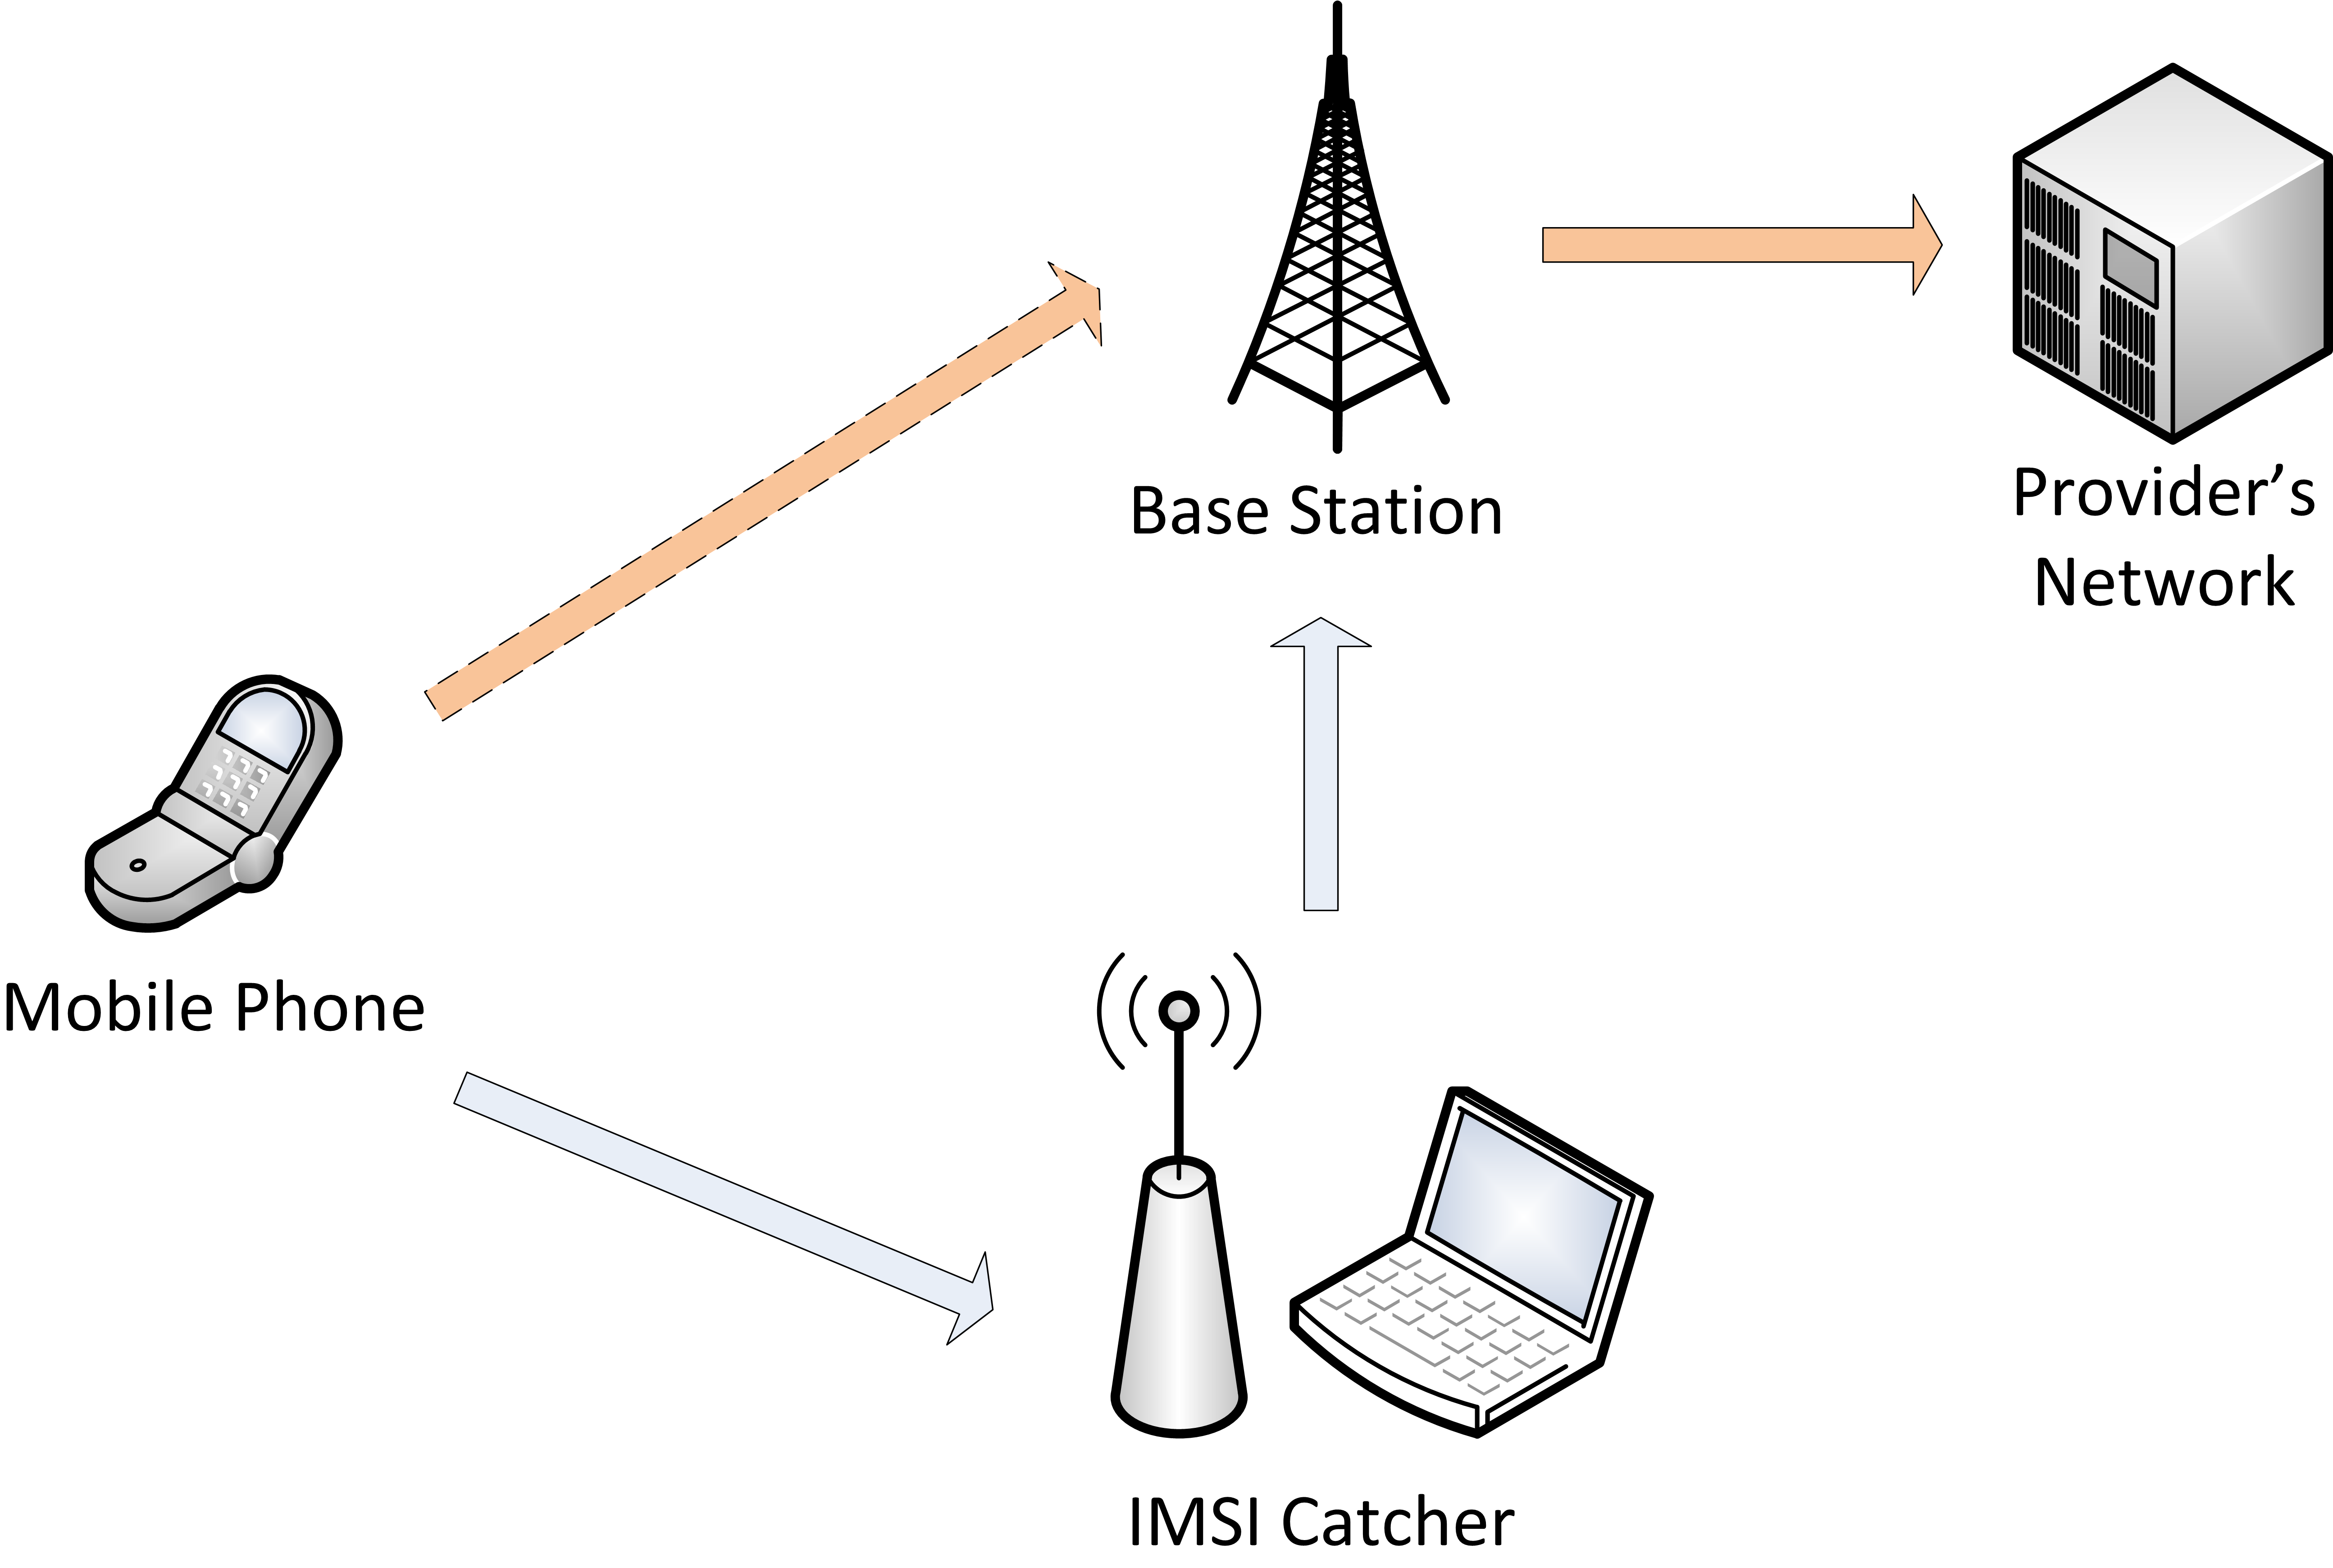
\includegraphics[width=.9\textwidth]{IMSICatcher}
\end{center}
\end{frame}

\begin{frame}{Threats}
\begin{block}{Technical Possibilities}
\begin{itemize}
	\item Tapping and recording of phone calls
	\item Localisation of subscribers
	\item Suppression of communication
\end{itemize}
\end{block}
Other concerns:
\begin{itemize}
	\item Cannot target individuals
	\item No emergency calls possible
	\item Procedural law situation
	\item Hard to prove operation in retrospect
\end{itemize}
... risk intensified by homebrew IMSI catcher projects!
\end{frame}

\subsection{IMSI Catcher Detection}
\begin{frame}{Detection}
Main Question: How to detect such a device?
\begin{itemize}
	\item<1-> Actively connect to the catcher
	\begin{itemize}
		\item<1-> Localisation possible once connected
	\end{itemize}
	\item<1-> \color<2>{red}Passively gather information
\end{itemize}
\vspace{.8cm}
\visible<2>{Procedure: Information that is publicly available
\begin{itemize}
	\item Broadcast Control Channel
	\begin{itemize}
		\item System Information Messages 1-4
		\item SI 1 and 2 of special interest
	\end{itemize}
	\item Parameters that can be measured
\end{itemize}
}
\end{frame}

\begin{frame}{Parameters}
Parameters measured:
\begin{itemize}
	\item Signal Strength
\end{itemize}
\vspace{.3cm}
Parameters harvested from SI:
\begin{itemize}
	\item ARFCN
	\item Country and Provider Codes
	\item Cell ID and Location Area Code
	\item Neighbouring Cell List
	\item Base Station Identification (not yet used)
\end{itemize}
\begin{alertblock}<2>{Main Problem}
Parameters that can be set, can be forged!
\end{alertblock}
\end{frame}

\tocsection{Current State}
\subsection{Architecture}
\begin{frame}{Overview}
\begin{center}
	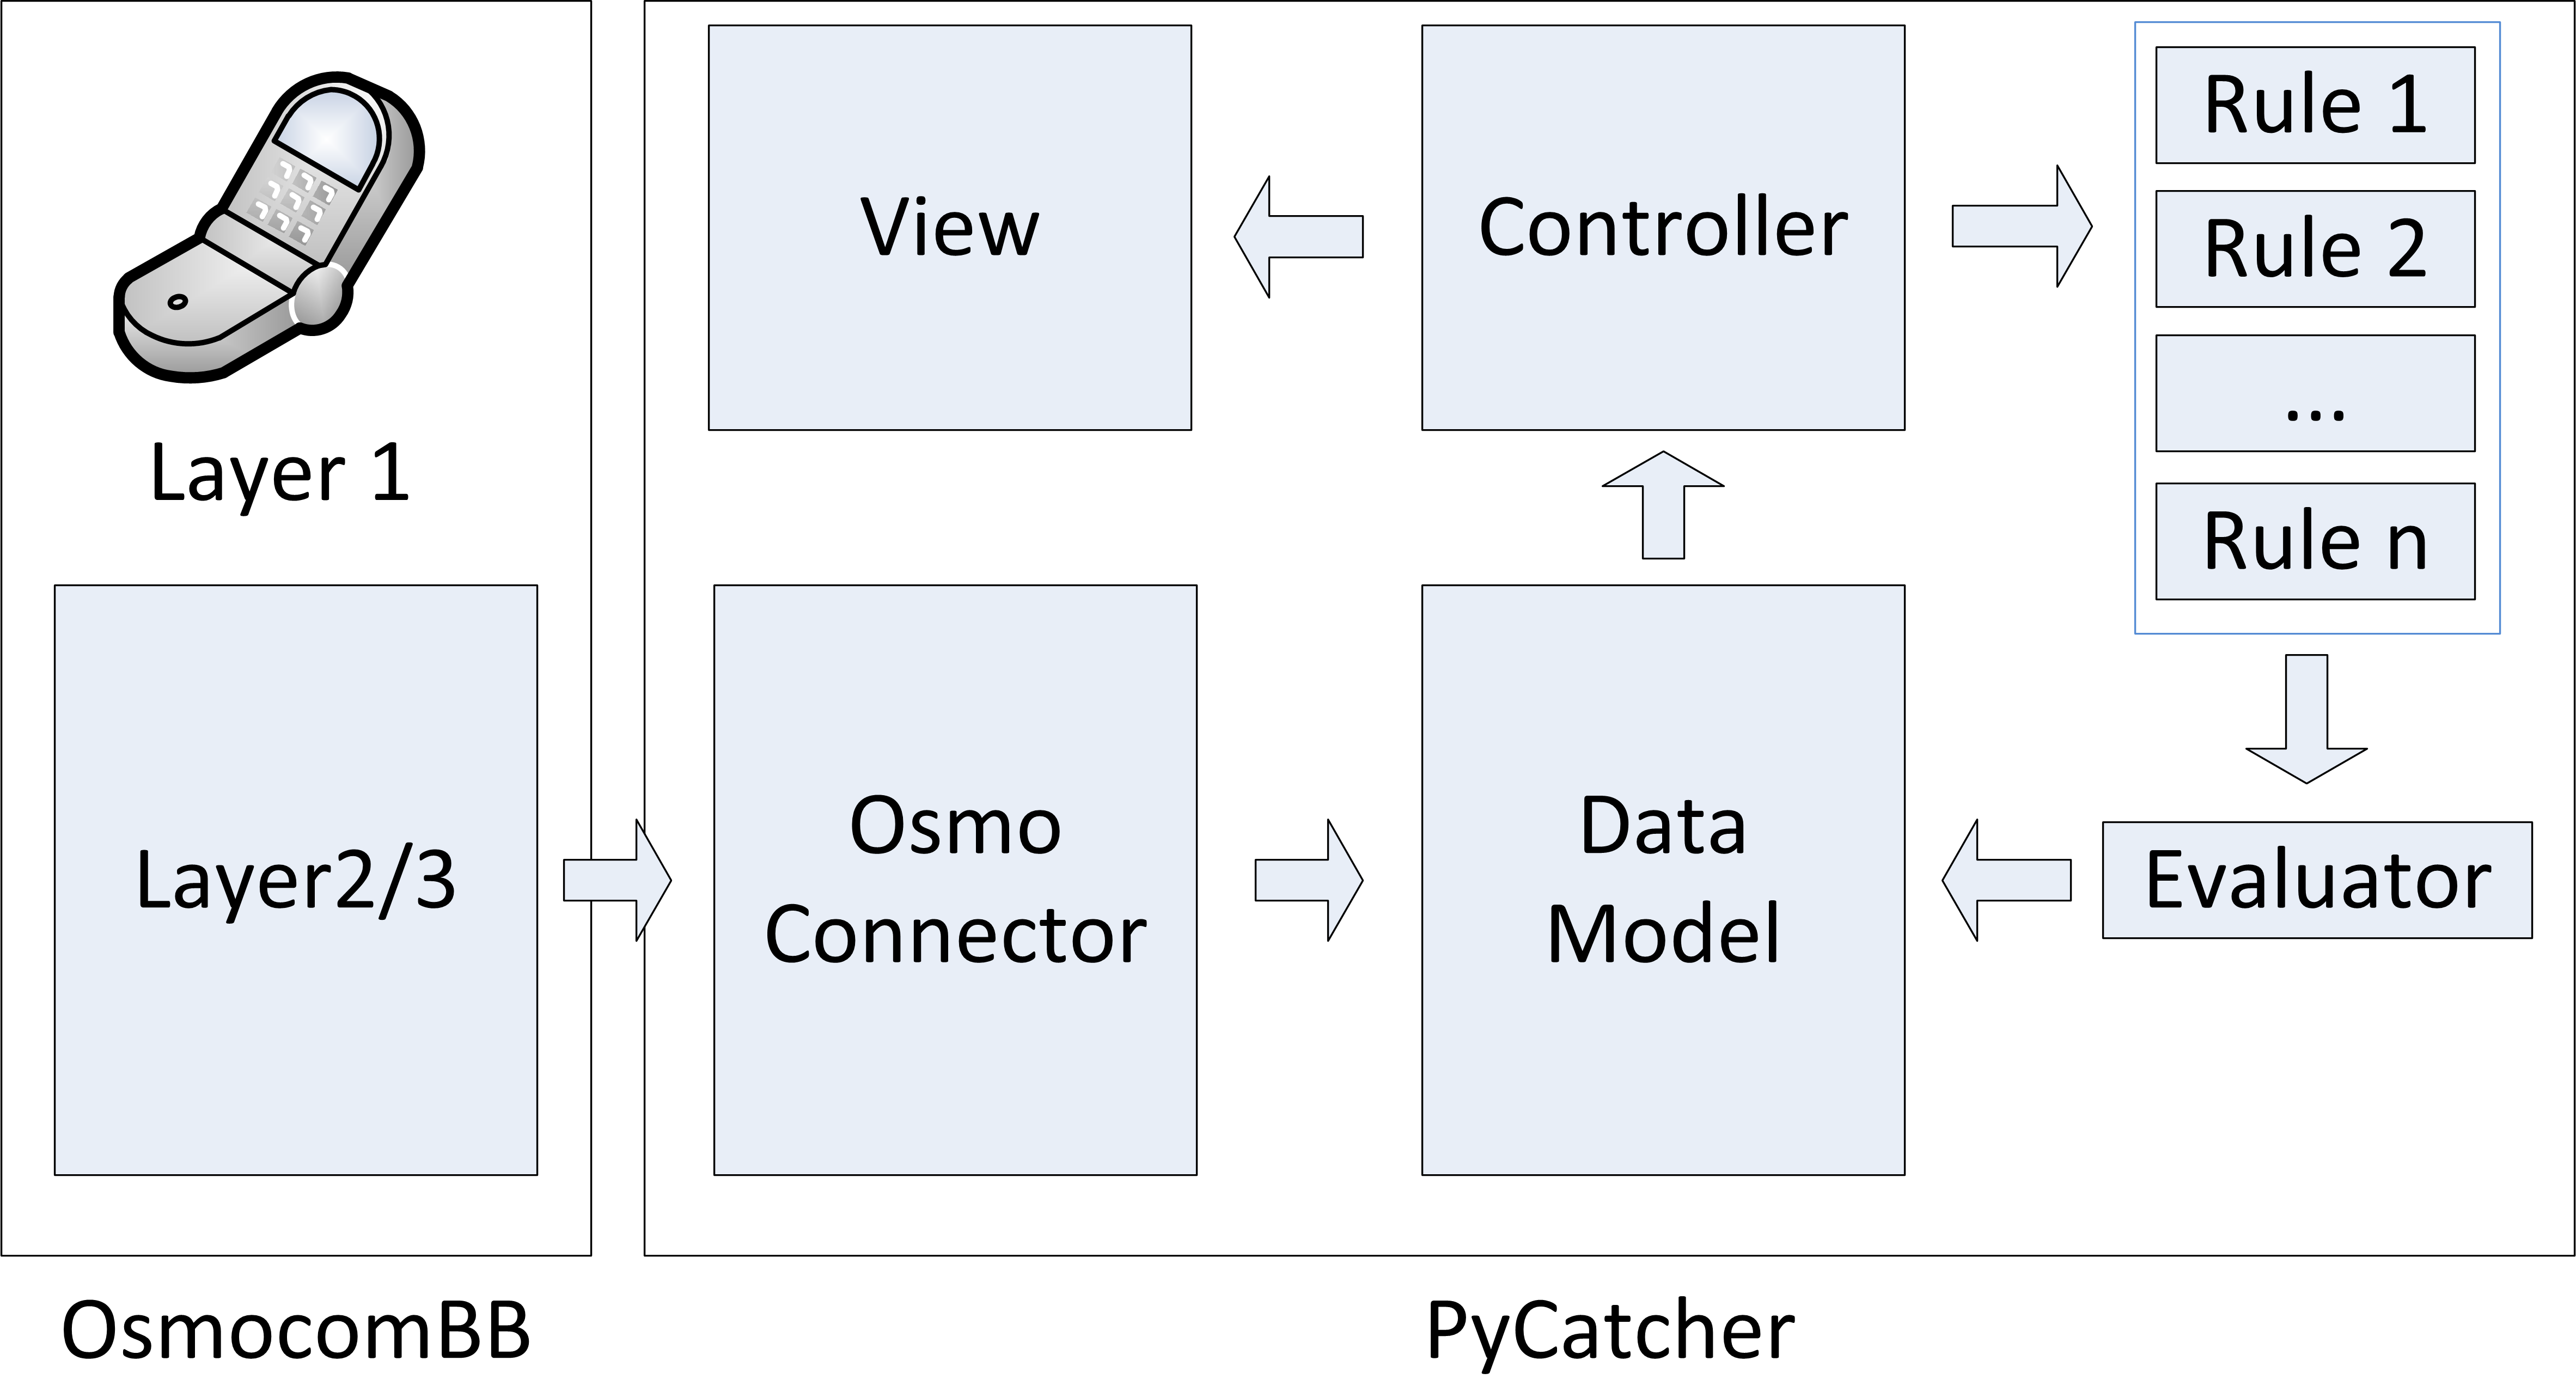
\includegraphics[width=\textwidth]{Architecture}
\end{center}

\end{frame}

\begin{frame}{Components}
Model/View/Controller oriented design with plug-in rules and evaluators
\begin{itemize}
	\item Data Model:
	\begin{itemize}
		\item Constantly updated by the OsmocomBB Framework
	\end{itemize}
	\item Rules:
	\begin{itemize}
		\item Mapping: $\text{DataModel}~\rightarrow~\{\text{Ok}\vert\text{Warning}\vert\text{Critical}\}$
		\item Different kinds of rules
		\item Constant re-evaluation
	\end{itemize}
	\item Evaluators:
	\begin{itemize}
		\item Gathers and aggregates rule results for a base station
		\item Conservative Evaluator
	\end{itemize}
\end{itemize}
\end{frame}

\subsection{Rules}
\begin{frame}{Rules}{Parameter Mapping and Context Rules}
Parameter Mappings:
\begin{itemize}
	\item Simple implication rules
	\item Mapping of parameter to range
	\item Integrity checks on single base stations
\end{itemize}
Context Rules:
\begin{itemize}
	\item Compare parameters with surrounding base stations
	\item See how well a base station fits in its neighbourhood
\end{itemize}
\begin{exampleblock}{Examples}
\begin{itemize}
	\item Check whether the ARCFN is in the registered range of the respective provider
	\item Check whether LAC is consistent with neighbouring LACs
\end{itemize}
\end{exampleblock}
\end{frame}

\begin{frame}{Rules}{Neighbourhood Rules}
Analyse the structure of the neighbourhood graph:
\begin{center}
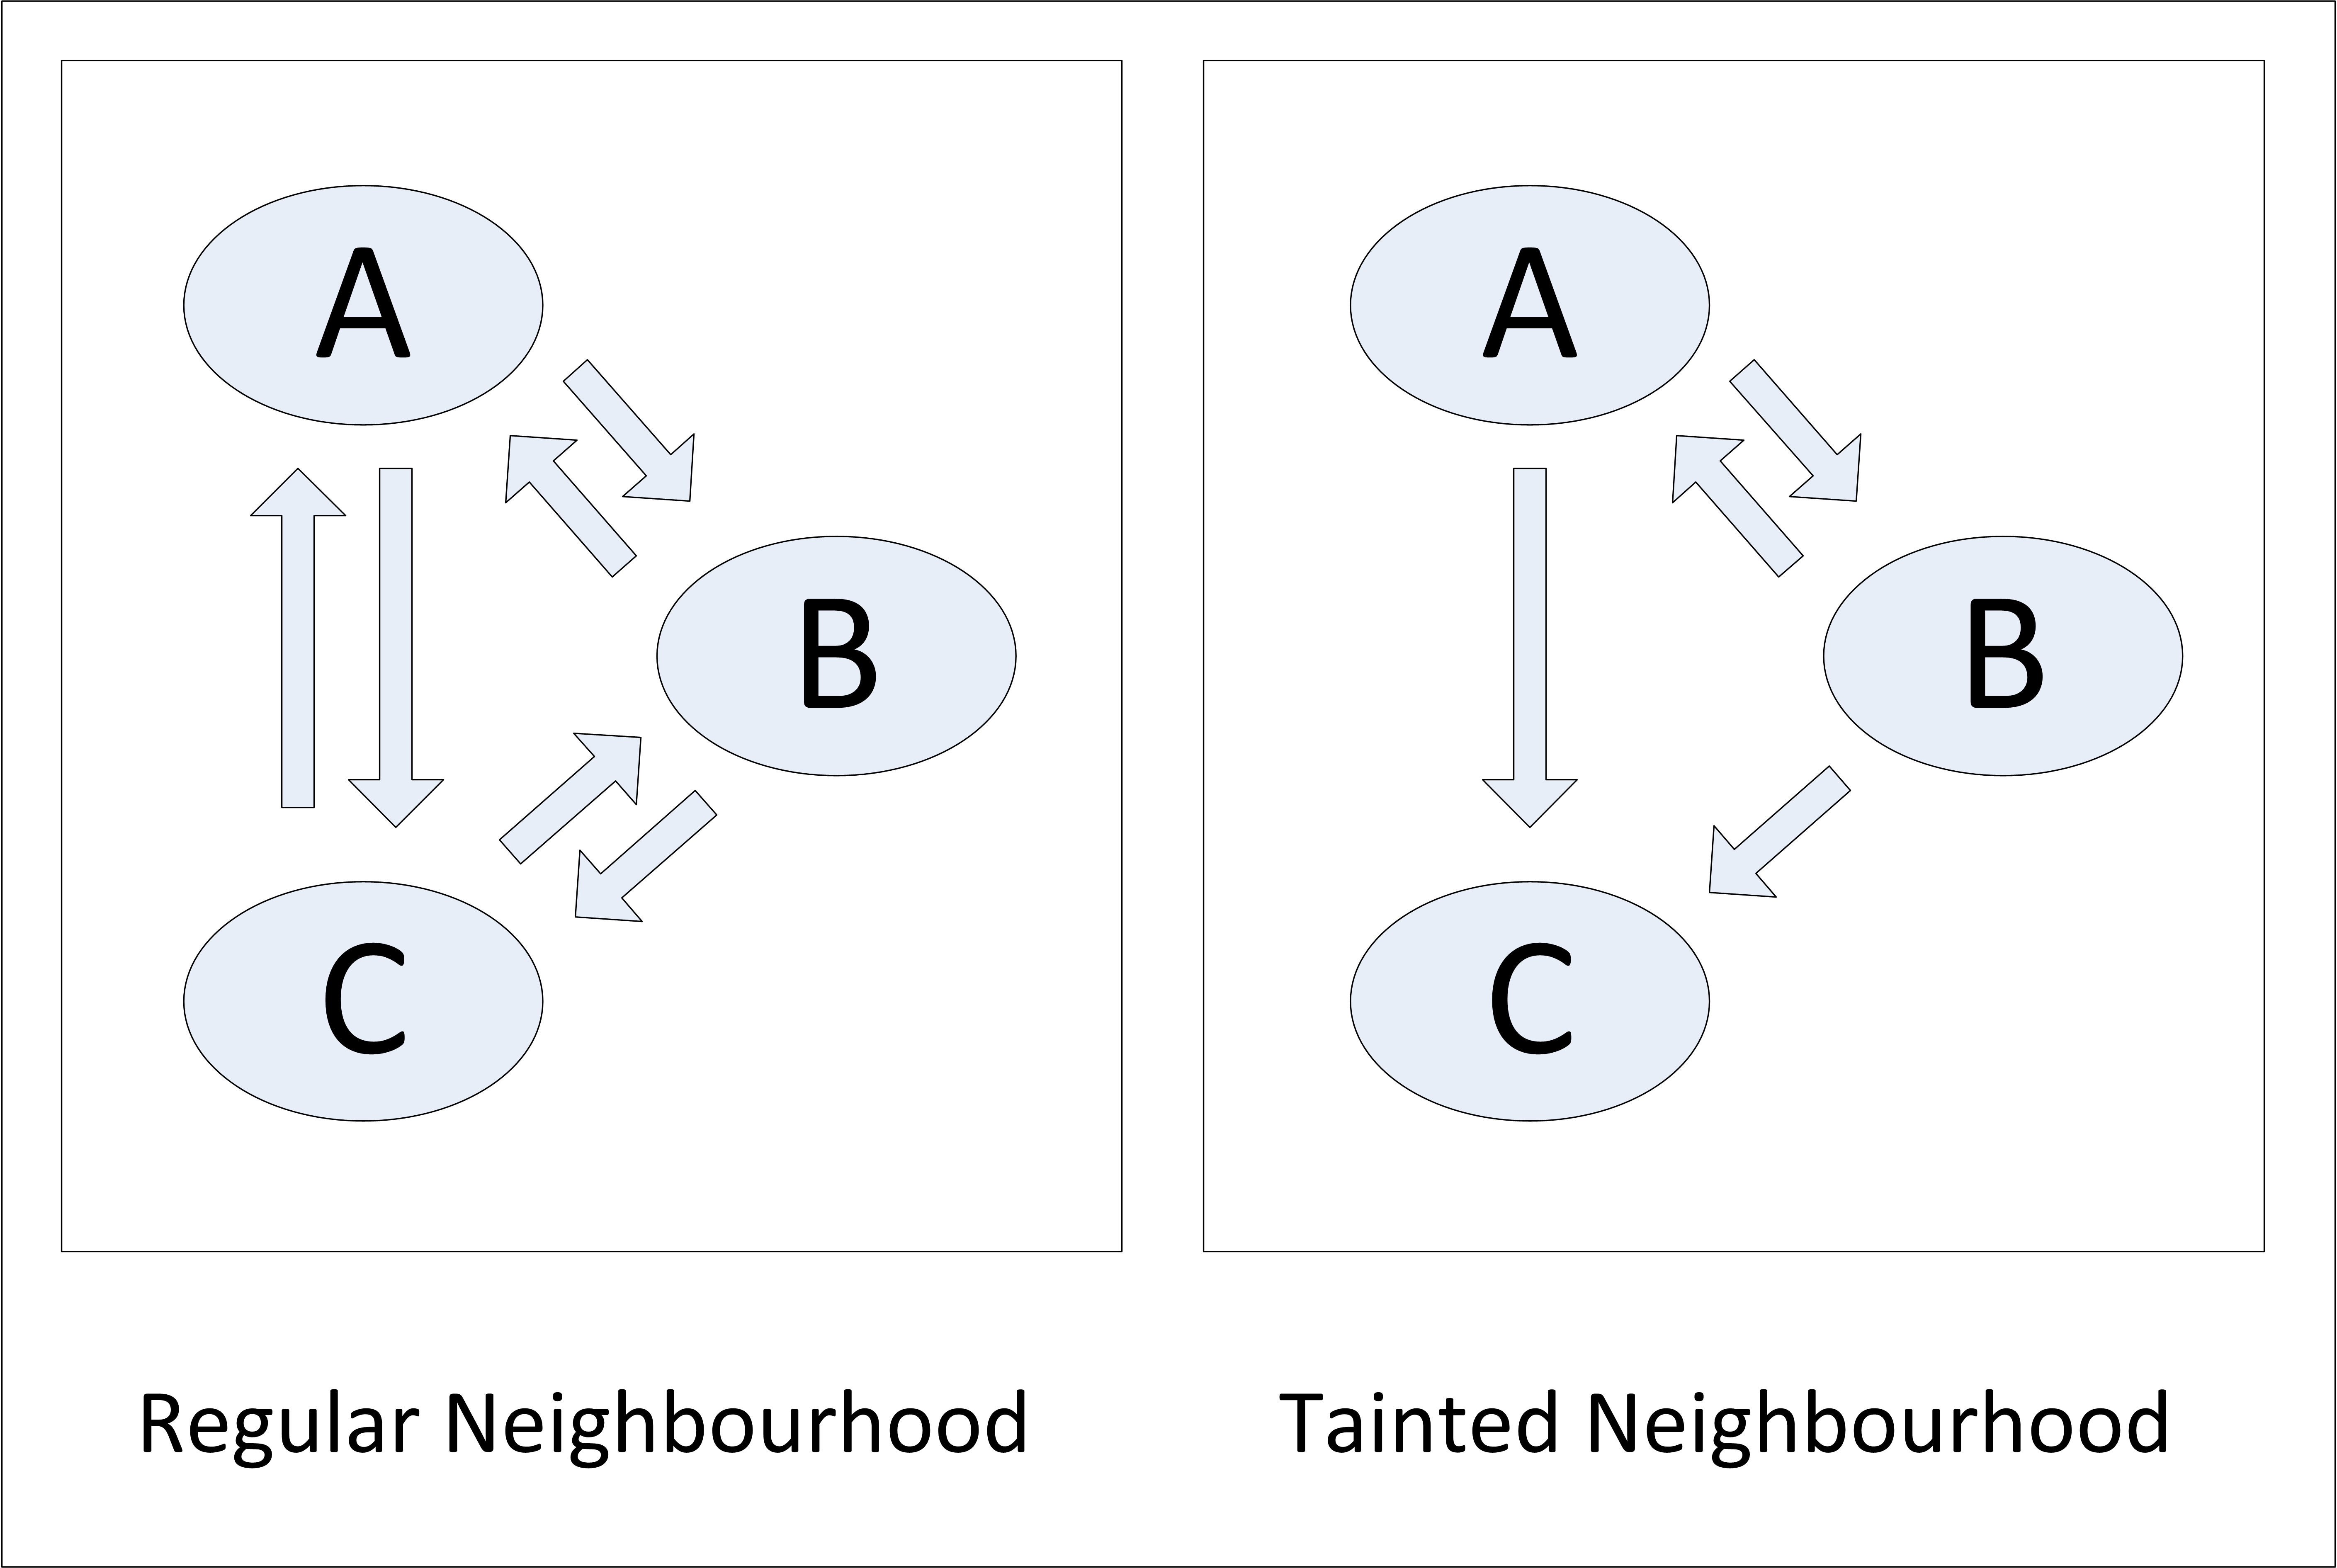
\includegraphics[width=.9\textwidth]{Neighbours}
\end{center}
\end{frame}

\tocsection{To Do}
\subsection{Rules}
\begin{frame}{Rules}{Databases}
\begin{alertblock}{Problem}
Forged parameters!
\end{alertblock}
Possible solution:
\begin{itemize}
	\item Cell ID Databases:
	\begin{itemize}
		\item Many official and open databases (Nokia/OpenCellID)
		\item Used for localisation, but can also be used vice versa!
	\end{itemize}
	\item Local Area Database:
	\begin{itemize}
		\item Learn surroundings
		\item 'Trustworthiness Score'
		\item Can use signal strength
	\end{itemize}
\end{itemize}
\end{frame}

\subsection{Evaluators}
\begin{frame}{Evaluators}{Bayes Filter}
\begin{block}{Bayesian Filtering}
A statistical algorithm that can be used to predict the class of an object given certain evaluations and base probabilities.
Uses Bayes theorem:
\[P(A\vert B)= \frac{P(B\vert A) \cdot P(A)}{P(B)}\]
\end{block}

\begin{exampleblock}{Bayes for a single Rule}
\[P(\text{B1 is catchter}\vert \text{R1 yields warning})\] 
\[=\frac{P(\text{R1 yields warning}\vert \text{B1 is catchter}) \cdot P(\text{B1 is catchter})}{P(\text{R1 yields warning})}\]
\end{exampleblock}
\end{frame}

\begin{frame}{Evaluators}{Bayes Filter (contd.)}
Bayes Theorem is recursive:
\begin{itemize}
	\item Evaluate P(B1 is catcher$\vert$R1 yields warning, R2 yields ok, $\ldots$)
	\item Further refinement possible:
	\begin{itemize}
		\item Refine base probabilities (enlarge database)
		\item Finer grained rule results than only three classes
		\item $\ldots$
	\end{itemize}
\end{itemize}
\end{frame}

\tocsection{Demo}
\subsection{Demo}
\begin{frame}{Demo}
\begin{center}
	\huge{Demo}
\end{center}
\end{frame}

\begin{frame}{The End}
\begin{center}
	\huge{Thank you for your attention! Questions?}
\end{center}
\end{frame} 

\end{document}

